\documentclass[11pt]{article}

\usepackage[backend=bibtex]{biblatex}
\usepackage[utf8]{inputenc}
\usepackage{amsmath}
\usepackage{amssymb}
\usepackage{anysize}
\usepackage{graphicx}
\usepackage{subcaption}
\graphicspath{ {./images/}, {./parts/igor/} }
\usepackage{color}
\usepackage{xcolor}
\usepackage{algorithm2e}
\usepackage{pgfplots}
\usepackage{hyperref}
\usepackage{booktabs}
\usepackage{tabularx}
\usepackage{titlesec}
\usepackage{array}
\usepackage{listings}
\bibliography{bibliography.bib}

\usepackage{tikz}
\usetikzlibrary{shapes,arrows}

\definecolor{mygreen}{rgb}{0,0.6,0}
\definecolor{mygray}{rgb}{0.5,0.5,0.5}
\definecolor{mypurple}{rgb}{0.58,0,0.82}


\usepackage{caption}
\DeclareCaptionFont{white}{\color{white}}
\DeclareCaptionFormat{listing}{\colorbox{gray}{\parbox[c]{\textwidth}{#1#2#3}}}

\setlength\parindent{0pt}
\setlength{\parskip}{10pt}

\marginsize{2cm}{2cm}{1cm}{1cm}
% % % % % % % % % % % % % % % % % % % % % % % % % % % % % % % % % % % % % %
% % % Commands
\titleformat{\paragraph}
{\normalfont\normalsize\bfseries\space}
{}
{0pt}
{}

% % % % % % % % % % % % % % % % % % % % % % % % % % % % % % % % % % % % % %
% % % Document start
\begin{document}

%  Title and authors
   \begin{center}
     {\huge\bfseries B31XP Robotics project\\ Robotic object follower}\\
      \vspace{2ex}
      \textsc{Andrey Pak, Donatas Kozlovskis, Enric Cornellà,\\ Fernando Garcia,  Igor Peric}
   \end{center}
   \vspace{2ex}%

%  Abstract
\begin{abstract}
This project presents a small, easy to build low-cost robot system, that is able to find coloured signs on the floor and implement the associated actions, e.g. stop, turn, pause, etc.
The robot hardware uses Raspberry Pi to control a set of motors, sensors and servo actuators. 
Report provides information about done review the hardware design and implementation of software using open source tools as C++ and OpenCV libraries. 
\end{abstract}

\section{Introduction}
\label{sec:intro}

Nowadays automation and robotics are leaving the traditional sectors as industrial manufacturing and becoming a part of daily life. It is integrating into our society, while many members still do not have a knowledge of it, since they are only familiar with the form of automation learned from massive social media.
Because of this trend of automation, it is important that educational organizations start preparing not only robotic researchers and designers, but also industrial personnel, who will be able
to take care of the robotic devices existing in our daily environment. 

A broad variety of robotic courses offered by universities or by massive open online education systems, increased during the past several years. However young students still lack opportunities to get hands-on experience on the understanding working principles, fabrication and implementation of robotic devices, which leads to the gap between theoretical and practical domain knowledge.

This project covered developing a low-cost wheeled robot, which is intended to promoting the teaching of basic computer science in schools \footnote{\url{http://www.raspberrypi.org/picademy/}}. Initial hardware design was provided by project supervisor, with limitations of only having motors, distance sensor, LCD screen, camera and Raspberry Pi (RPi) single-board computer.
Constraint of  Raspberry Pi computation power raised challenge to find an  optimal techniques of implementing controllers of sensors and actuators, knowing that most of the resources are consumed by image processing to implement and realise desired robot actions. In this report, the optimal software design procedure is presented leading to the working example of constructed robot.


\section{Description of the Project}
The present section describes the different stages of the project; design, management, software implementation and hardware improvement. It also presents the main goals of the work as well as a brief description of the main sections which compose this document.

As it has been presented in section \ref{sec:intro}, the main goal of the project is to introduce robotics in general and open-source tools such as Raspberry Pi in a dynamic and friendly manner in order to enhance the learning experience and engage children. It has been proved that the most suitable way to achieve this is to present the activity as an interactive game \url{ http://psycnet.apa.org/index.cfm?fa=search.displayRecord&uid=1999-02807-000}

Considering the importance of self-motivation in whatever successful learning process, it is important to assure an enjoyable experience for the user. However, to be able to produce a pleasant and reinforced experience is conditioned by the field studied. For this reason this topic is worth it to be studied.

The main goal is to provide an independent robot platform able to interact with the user, in this case children. This idea not only forces the implementation to be as robust as possible, but also to implement a strong feedback component in order to give the impression to the user what is going on in every single moment during the game development. It is so important to assure the reduction of uncertainty moments produced by an expected reaction of the system as well as a lack of information during the actions performed. 

Firstly, and according to the previous statement, a robust interaction method needs to be defined because will provide to the user the control of the system in a reliable way. An intuitive technique to do this is to make the robot able to recognize different signs and execute the correspondent actions when one of these signs are presented. The basic signs are an arrow, a cross and a circle but it can be easily extended to more. Showing this bunch of signs to the platform, children should be able to give the appropriate instructions to move it from point A to point B.

Secondly, the concept of feedback in every single moment is essential. It will provide the current state of the process, reinforcement or additional guidance to continue the experience. In this way, two different types of feedback are defined: Acoustic and visual. 

The first type of feedback is provided using a set of representative sounds that describes 'how the robot feels'. They represent states such as uncertainty, sign found, following mode, executing action and game over. The second type of feedback is provided through text displayed in a LCD screen guiding the user in any situation.

The main challenge of this project is to be able to segment the sign properly under different light conditions and surfaces, but also taking into account the limited computational power of the Raspberry Pi (in this sense a comparative with another board is provided). One important improvement to accomplish successfully this goal is the replacement of the camera installed for an IR camera. The fusion of the IR information provides a better sign recognitions under certain bad light conditions. Since the robot has to be able to move autonomously in any flat surface, it is also equipped with a proximity sensor for collision detection and two independent motors.

To conclude this section, a brief summary of the different sections presented in the report is provided. 


\section{State of the art}

\section{Project Management}

In order to have a continuous progress, project management had to be established. The goal of management is to ensure that the whole project and software development process works as it is intended, allowing project activities to meet project requirements.

The main steps of project management process are initiating, planning, executing, monitoring and controlling, and closing. Thus firstly, project team meetings were established on a weekly basis. Continuing defining the project goals, tight control of timeline had to be set as well, in order to keep track of deadlines.

For this purpose the Gantt charts web tool\footnote{\url{https://teamgantt.com/}} was employed. It allowed to breakdown work structure of the project to small tasks, setting the start and finish dates individually. An example of Gantt chart used in this project can be seen in figure \ref{fig:gannt_example}.

\begin{figure}[ht!]
	\centering
	\includegraphics[width=1\textwidth]{gantt_chart_part}
	\caption{Part of planning represented on Gantt chart}
	\label{fig:gannt_example}
\end{figure}

Beside the track of the tasks, version control system for tracking the code changes had to be chosen. Common tools are Team Foundation Version Control, Mercurial or Git source control. Due to affordability and compatibility, distributed version control system Git was chosen. 

For hosting the central GIT repository the two main players are \textit{Github} and \textit{Bitbucket}.
The main difference between the two is being cost for non-open source projects. \textit{Bitbucket} is free for teams up to 5 users and can host private closed source repositories whereas \textit{Github} does not provide private repositories for free. Thus the specifications of providers led to choose \textit{Bitbucket} for being web-based hosting service for this project.

After setting up source version control, actual developing had started. In order to keep track with the Gantt chart, specific issues were created and assigned to each team member on a weekly basis. Project management tool \textit{Bitbucket Cards}, a part of \textit{Bitbucket}, offered interaction with issues on one easy-to-use, intuitive dashboard, where progress of tasks from one list to the next was easy to track. An example of early stage project board can be seen in figure \ref{fig:bitcards}.

\begin{figure}[ht!]
	\centering
	\includegraphics[width=1\textwidth]{bitbucket_cards}
	\caption{Early stage project board}
	\label{fig:bitcards}
\end{figure}

All mentioned tools were employed until the end of the project, resulting on continuous development and progress.

\section{Implementation}
\clearpage
\subsection{Overview}
\subsection{Hardware}
	The list of robot's main hardware components is as follows:

\begin{itemize}
  \item Raspberry Pi Model B Board (see Fig. \ref{fig:rpi_board})
  \item Raspberry Pi No-IR Camera
  \item RD02 Robot drive system
  \item Ultrasound Proximity sensor
  \item $I^2C$ Breakout Board
  \item LCD screen
\end{itemize}

\begin{figure}[h!]
\centering 

	\begin{subfigure}[h]{0.35\textwidth}
		\centering
			\includegraphics[width=\textwidth]{rpi.png}
			\subcaption{Raspberry Pi Model B board}
			\label{fig:rpi_board}
	\end{subfigure}
	\begin{subfigure}[h]{0.35\textwidth}
		\centering
			\includegraphics[width=\textwidth]{noir.png}
			\subcaption{Raspberry pi NoIR camera module}
			\label{fig:rpi_noir}
	\end{subfigure}

\caption{Raspberry Pi and NoIR camera}
\label{fig:rpi}
\end{figure}

\subsubsection{Mechanical Part} 

The robot drive unit RD02 used in this project consists of MD25 motor control
board, two EMG30 modules (motor, gearbox and a mounting bracket) and two 100mm
wheels\cite{robotel} (see Fig. \ref{fig:rd02}).

The frame of the robot consists of aluminum profiles and a perforated plate that
serves as a base for mounting electronic components. Two driving wheels
are mounted on a EMG30 gearbox shaft that connected to the frame via the
provided bracket. A metal ball wheel is located in front of the robot and
provides remaining support.

EMG30 is a module that incorporates motor, gearbox and encoder with Hall sensor.
It is suited for medium robotics applications. The gearbox provides increased
torque allowing robust movement in different environments while the Hall sensor
obtains information about the rotation of the shaft.

\begin{figure}[h!]
\centering 

	\begin{subfigure}[h]{0.35\textwidth}
		\centering
			\includegraphics[width=\textwidth]{rd02.png}
			\subcaption{RD02 Robot Drive System}
			\label{fig:rd02}
	\end{subfigure}
	\begin{subfigure}[h]{0.35\textwidth}
		\centering 
			\includegraphics[width=\textwidth]{lcd.png}
			\subcaption{20x4 LCD Module and ultrasonic range sensor}
			\label{fig:lcd_us}
	\end{subfigure}

\caption{RD02 Robot Drive System}
\label{fig:modules}
\end{figure}

\subsubsection{Electronics}
 
The main electronic component of the robot is the Raspberry Pi Model
B single-board computer. Its technical specifications are listed in the Table
\ref{tab:rpi_specs}.

\begin{table}[h!]
	\setlength\extrarowheight{2pt}
    \begin{tabularx}{\textwidth}{XX}
   	\toprule
	    \textbf{System on a chip}  & Broadcom BCM2835                                            \\
	    \textbf{CPU  }             & 700 MHz ARM11                                               \\
	    \textbf{GPU}               & Broadcom VideoCore IV @ 250 MHz                             \\
	    \textbf{RAM}               & 512 Mb shared with GPU                                      \\
	    \textbf{Memory}            & SD Card Slot                                                \\
	    \textbf{Ports}             & 2x USB, LAN, 3.5mm phone jack, HDMI,  GPIO (UART, $I^2C$, SPI) \\
	    \textbf{Power Consumption} & 700 mA (3.5 W)                                              \\
    \bottomrule
    \end{tabularx}
    \caption{Raspberry Pi Model B Specifications}
    \label{tab:rpi_specs}
\end{table}

The board is running an adapted version of the Debian Linux distribution. The
development can either be performed on the board itself after connecting the
necessary peripherals, or via remote connection such as SSH.

The board is powered using 11.1V Turnigy LiPo Battery via power adapter that
splits the voltage into 12V (motors) and 5V lines. According to the external
power supply measurements, the average total consumption during movement is
approximately 8W.

The Raspberry Pi peripherals include a WiFi adapter, GPIO breakout board for
simplifying the connection of other modules, and a Raspberry Pi camera (see
Fig. \ref{fig:rpi_noir}).
RPi camera is a board-specific 5Mp camera module connected via 15-pin MIPI (Mobile Industry
Processor Interface) connector. It is capable of capturing 1080p video and
perform basic hardware video processing. Two different types of cameras were
tested - standard camera and near-IR 'NoIR' camera with the infrared filter
removed.
The performance comparison of different cameras is shown in the Table
\ref{tab:cam_perf}.  In order to increase the reliability and robustness of 
NoIR camera, a couple of IR LEDs were installed to provide additional illumination.

After a series of experiments, the signs were made of a highly-reflective duct
tape that showed high reflectance under poor lighting
conditions. The usage of the NoIR camera accompanied with a couple of IR LEDs
showed high segmentation performance with minimum lighting provided.

MD25 is a dual H-Bridge $I^2C$ / Serial motor driver suited for the control of
EMG30 modules.
It provides additional capabilities in the motor manipulation, such as variable
acceleration, motor current information and independent control of two motors
with encoder feedback. It is also equipped with a 5V regulator, however it is
impossible to power the Raspberry Pi as the continuous supply rate is 300 mA,
while the average consumption of Raspberry Pi is 700 mA.

Due to the reason explained before, Raspberry Pi is powered using Taco Power TSR
1-2450 DC-DC voltage step-down modules that provide 5V 1A output \cite{taco}.

% Fix table here
\begin{table}[h!]
	\setlength\extrarowheight{2pt}
	\setlength\arraycolsep{5pt}
    \begin{tabularx}{\textwidth}{XXXX}
    	\toprule
    	\bf
	    Resolution / Camera Setup & \bf Raspberry Pi (CPU) + Raspberry Pi Camera & \bf 
	    Raspberry Pi (CPU) + Logitech C270 & \bf  Odroid-U3 (CPU) + Logitech C270 \\
	    \hline
	    160x120            & 18           & 9          & 30         \\
	    320x240            & 6            & 4.8        & 20         \\
	    640x480            & 2.5          & 2.3        & 11         \\
	    1280x720           & 0.6          & 0.8        & 4          \\
	    \bottomrule
    \end{tabularx}
    \caption{Camera Performance comparison}
    \label{tab:cam_perf}
\end{table}

As can be seen from the Table \ref{tab:cam_perf}, the main advantage of using
RPi camera is its performance - it outperforms generic Webcam grace to hardware
optimization and, in particular, absence of resizing routine in the code.
However, the disadvantage lies in the specificity of the camera, that can only
be used on the RPi board, while the USB Webcam can be used everywhere, so in
order to port the solution to another platform, the camera change as well as
 code modification are required.

The robot is also equipped with an ultrasound proximity sensor used for obstacle
detection. It is a basic proximity sensor with a focus of 15 degrees and an
accuracy about 2 mm. An $I^2C$ LCD Screen module provides an interface for visual feedback.
These components are shown on the figure \ref{fig:lcd_us}.
	
\subsection{Software}


Conceptual overview of software architecture and its parts is given on figure \ref{fig:soft_overview}. All components will be discussed and described in detail in this section of the report. 

%\begin{figure}[th!]
%\center
%\includegraphics[scale=0.7]{images/software-architecture.png}
%\caption{Overview of software architecture of the solution}
%\end{figure}


\begin{figure}[!ht]
	\hspace{-1cm}
	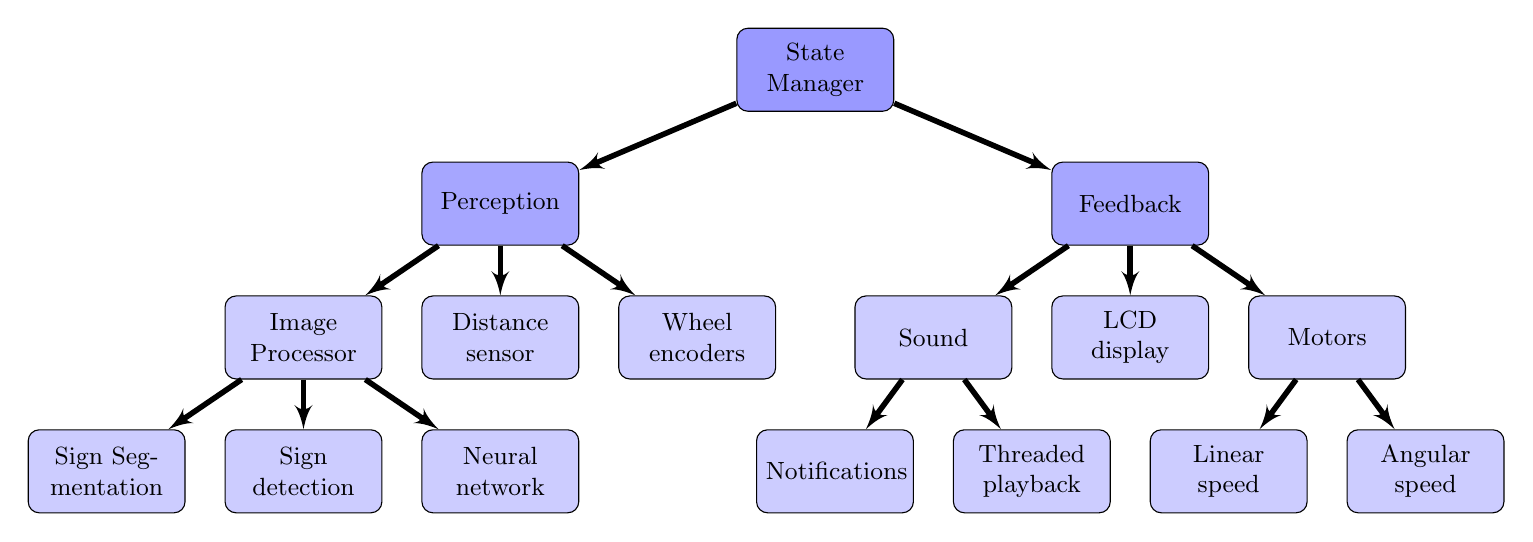
\begin{tikzpicture}[node distance = 2.5cm, auto]
	% % % % % % % % % % % % % % % % % % % % % % % % % % % % % %
	% Define styles
	\tikzstyle{block} = [rectangle, draw, fill=blue!20, text width=5em, text centered, 
					     rounded corners, minimum height=3em, font=\small]
	\tikzstyle{line} = [draw, -latex', line width =2pt]
	
	% % % % % % % % % % % % % % % % % % % % % % % % % % % % % %
	% Place nodes
	% parent
	\node [block,  fill=blue!40] (sm) {State Manager};
	% child level 1
	\node [block, fill=blue!35, below of=sm, node distance = 1.7 cm, xshift=-4.cm] (pc) {Perception};
	\node [block, fill=blue!35, below of=sm, node distance = 1.7 cm, xshift=4.cm] (fb) {Feedback};
	% child level 2 left
	\node [block, below of=pc, node distance = 1.7cm] (ds) {Distance sensor};
	\node [block, left of=ds] (ip) {Image Processor};
	\node [block, right of=ds,  node distance = 2.5 cm] (we) {Wheel encoders};
	% %third level left
	\node [block, below of=ip, node distance = 1.7 cm] (sgd) {Sign detection};
	\node [block, left of=sgd] (sgm) {Sign Segmentation};
	\node [block, right of=sgd] (nn) {Neural network};
	
	% child level 2 right
	\node [block, below of=fb, node distance = 1.7 cm] 						(ld) {LCD display};
	\node [block, left of=ld] 	(sn) {Sound};
	\node [block, right of=ld] (mt) {Motors};
	
	% %third level right
	\node [block, below of=sn, node distance = 1.7 cm, xshift=-1.25cm] (ntf) {Notifications};
	\node [block, below of=sn, node distance = 1.7 cm, xshift=1.25cm] (thr) {Threaded playback};
	% %third level right
	\node [block, below of=mt, node distance = 1.7 cm, xshift=-1.25cm] (lns) {Linear speed};
	\node [block, below of=mt, node distance = 1.7 cm, xshift=1.25cm] (ags) {Angular speed};
	
%	\node [block, right of=left,  node distance = 3 cm] (right) {Turn right};
	% Draw edges
	\path [line] (sm) -- (fb);
	\path [line] (sm) -- (pc);
	% %
	\path [line] (pc) -- (ip);
	\path [line] (pc) -- (we);
	\path [line] (pc) -- (ds);
	% %
	\path [line] (fb) -- (sn);
	\path [line] (fb) -- (mt);
	\path [line] (fb) -- (ld);
	% %  third level image proc
	\path [line] (ip) -- (sgm);
	\path [line] (ip) -- (sgd);
	\path [line] (ip) -- (nn);
	% %  third level sound
	\path [line] (sn) -- (ntf);
	\path [line] (sn) -- (thr);
	% %  third level motors
	\path [line] (mt) -- (lns);
	\path [line] (mt) -- (ags);
	\end{tikzpicture}
	\caption{Overview of software architecture of the solution}
	\label{fig:soft_overview}
\end{figure}



\subsubsection{State machine}


One of the most common and intuitive approaches for implementation of software controller for hardware system is state-machine approach. It is fairly simple concept, with only a couple of important considerations.

System controlled by state machine has certain number of possible, unique and well defined states that it can be in at every moment of execution. State defines the behaviour of the system in every discrete moment of time, including three important aspects: sensor data acquisition, output behaviour computation and state transition check. In other words, every state has it is own logic for doing all of these three mentioned steps, which gives a lot of variability for possible control scenarios. It is worth mentioning that some states might skip certain steps or perform some steps more than once without state transition check, for example.

\paragraph{System states}

At any moment of time robot can be in one of the following state seen in figure \ref{fig:algorithm-diagram}.

\begin{figure}[ht!]
	\centering
	\includegraphics[width=0.7\textwidth]{newDiagram.png}
	\caption{State transition algorithm}
	\label{fig:algorithm-diagram}
\end{figure}

\textit{IDLE} state sets both angular and linear speed to zero and waits for any of the segmented object currently inside view to go away, after which it goes to WIGGLING state.

\textit{WIGGLING} state rotates the robot around its vertical axis with constant angular and zero linear speed until a sign is detected. After detecting a sign it switches to APPROACHING\_SIGN state.

\textit{APPROACHING\_SIGN} state moves the robot close to the sign it has seen in the previous state. It does this by setting the linear speed to constant value and adjusting angular speed all the time based on the horizontal position of the target sign in the view. Robot will move in the direction needed to align the sign to the center of the screen, and it will do that proportionally to the distance of the target to the center.

\textit{EXECUTING\_COMMAND} state has different behavior depending on the type of the sign that was seen in the state before. If it was goal sign, it will switch to the GAME\_OVER state and the game will end. If it was stop sign, robot will just wait for certain predefined time-out (5 seconds) and switch to state MARCHING\_FORWARD. If it was the arrow sign, robot will turn desired angle and switch switch to state MARCHING\_FORWARD.

\textit{MARCHING\_FORWARD} state sets the linear speed to constant and angular to zero. In this state robot constantly monitors camera image stream and can potentially switch to APPROACHING\_SIGN state once a sign is detected in perceptive area of the image.

\textit{GAME\_OVER} state is entered after goal sign is approached. After displacing notification about game completion (through audio and visual feedback), robot remains idle until hardware button is pressed for the start of the new game.

%\begin{figure}[th!]
%	\centering
%	\includegraphics[scale=1]{algorithm-diagram.png}
%	\caption{State transition algorithm}
%	\label{fig:algorithm-diagram}
%\end{figure}

%\paragraph{Sensor data acquisition}

First step in state machine control loop is sensor acquisition step. If possible, data is acquired from all input sensors in order to determine current state of the environment. This includes acquisition of camera image using OpenCV, reading heading angle from motor driver and reading distances from ultrasonic sensor driver.

Last values of all the readings are always stored in local members of the class, so they can be referenced between successive acquisitions.

%\paragraph{Output behavior computation}

Based on the sensed input data values for all output units are being calculated. This includes linear and angular wheel velocities, message for LCD display, sound to be played on speakers, etc.

%\paragraph{State transition condition}

Every state has to have clearly defined condition which will make the system switch to any of the other states. System remains in the current state until one of the state transition conditions has been met.





\subsubsection{Actuators and sensing drivers}
Most of the processes the robot is doing need either to get some information from external sensors or to send data to the actuators or displays. Whenever this happens the robot needs to be able to communicate with external gadgets using drivers.

In this part the sound, lcd and proximity sensor will be explained.

The first one is built directly on RaspberryPi. Since the platform has already an output of 3.5mm there is no need to communicate with any other. However it is considered as an external gadget because a speaker is needed. \textit{Explanation of libraries used for doing this.}

The second and the third (lcd and proximity) have a little microprocessor in them. This forces the robot to use a communication protocol in order to exchange information with them.

LCD display is used in order to show information about the current state of the robot. Is a very powerful way to know what the robot is thinking or doing without the need of connecting a screen to the raspberryPi. This is very important since the less computational power expended on the RP the better. Avoiding the initialization of a graphical user interface will result in a slightly more fast execution of the program, which is desired.

Proximity sensor will give information to the robot about its surroundings. The working principle is based on ultrasonic sounds that rebound on objects. By calculating the amount of time for a sound wave to get back to the sensor it is possible to estimate the distance.

The two last gadgets use both the $i^{2}c$ protocol in order to communicate with the raspberryPi. $I^{2}c$... blablabla Drivers extracted from robo-electronics.

HOW TO WRITE RASPBERRY PI

WHO IS EXPLAINING THE I2C DEEPLY?

\subsubsection{Motion module}
This module connects desired action behaviour via the control of  robot wheels. Since designed robot uses
Dual 12Volt 2.8Amp H Bridge Motor Drive MD25 \footnote{\url{http://www.robot-electronics.co.uk/htm/md25i2c.htm}} board, controlling the wheels was accomplished using $I^2C$ bus system mode.
Generally this module had to realize following actions:
\begin{itemize}
	\item Drive motors by setting individual speeds for both wheels.
	\item Get heading of the robot by reading encoder values.
\end{itemize}
These requirements led to splitting the whole module into two blocks:  one being responsible for driving motors and another for reading/writing encoders.

\begin{figure}[!ht]
	\centering
	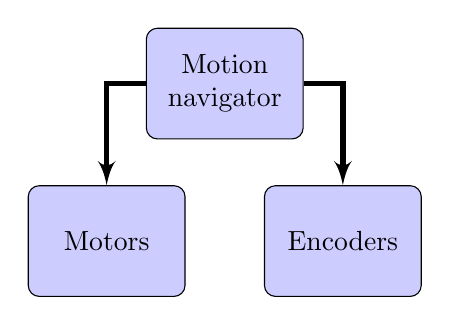
\begin{tikzpicture}[node distance = 2cm, auto]
	\tikzstyle{block} = [rectangle, draw, fill=blue!20, 
	text width=5em, text centered, rounded corners, minimum height=4em]
	\tikzstyle{line} = [draw, -latex', line width =2pt]
	% Place nodes
	\node [block] (navigator) {Motion navigator};
	\node [block, below of=navigator, xshift=-1.5cm] (motors) {Motors};
	\node [block, below of=navigator, xshift= 1.5cm] (encoders) {Encoders};
	% Draw edges
	\path [line] (navigator) -| (motors);
	\path [line] (navigator) -| (encoders);
	\end{tikzpicture}
	\caption{Motion module structure}
	\label{fig:motion_structure}
\end{figure}

\paragraph{Controlling motors}

All communications between high level functions and motors were realized via  $I^2C$ bus command register.
The MD25 has 17 registers numbered 0 to 16 as follows:
\begin{table}[!h]
	\centering
	\scalebox{0.9}{
		\begin{tabular}{@{}llll@{}}
			\toprule
			\textbf{Register} & \textbf{Name}     & \textbf{Read/Write} & \textbf{Description}                                             \\ \midrule
			0                 & Speed1            & R/W                 & Motor1 speed (mode 0,1) or speed (mode 2,3)                      \\
			1                 & Speed2/Turn       & R/W                 & Motor2 speed (mode 0,1) or turn (mode 2,3)                       \\
			2                 & Enc1a             & Read only           & Encoder 1 position, 1st byte (highest)   \\
			3                 & Enc1b             & Read only           & Encoder 1 position, 2nd byte                                     \\
			4                 & Enc1c             & Read only           & Encoder 1 position, 3rd byte                                     \\
			5                 & Enc1d             & Read only           & Encoder 1 position, 4th (lowest byte)                            \\
			6                 & Enc2a             & Read only           & Encoder 2 position, 1st  byte (highest)  \\
			7                 & Enc2b             & Read only           & Encoder 2 position, 2nd byte                                     \\
			8                 & Enc2c             & Read only           & Encoder 2 position, 3rd byte                                     \\
			9                 & Enc2d             & Read only           & Encoder 2 position, 4th byte (lowest byte)                       \\
			10                & Battery volts     & Read only           & The supply battery voltage                                       \\
			11                & Motor 1 current   & Read only           & The current through motor 1                                      \\
			12                & Motor 2 current   & Read only           & The current through motor 2                                      \\
			13                & Software Revision & Read only           & Software Revision Number                                         \\
			14                & Acceleration rate & R/W                 & Optional Acceleration register                                   \\
			15                & Mode              & R/W                 & Mode of operation (see below)                                    \\
			16                & Command           & Write only          & Used for reset of encoder counts and module address changes      \\ \bottomrule
		\end{tabular}
	}	
	\caption{The MD25 register values and description}
	\label{table:md25}
\end{table}

\newpage
For controlling the motors, registers 0, 1 and 15 are used. Firstly, initializing motor control, mode register (15) is modified.
The mode register selects which mode of operation and $I^2C$ data input type the user requires. Here the type 3 was chosen and writing this value 
to the mode register makes enables turn mode: 'speed1' controls both motors \textit{speed}, and 'speed2' becomes the \textit{turn} value. 
These two values correspond to the \textit{linear} and \textit{angular} respectively, which are provided by state machine.
Data is in the range of -128 for full reverse, 0 for stop and 127 for full forward speed of motors.

It is worth to mention, that turn mode looks at the speed register to decide if the direction is forward or reverse. Then it applies a subtraction or addition of the turn value on both motors. If the direction is forward:
\begin{table}[!ht]
	\centering
	\begin{tabular}{lcl}
		motor speed1 & = & speed - turn,\\
		motor speed2 & = & speed + turn,
	\end{tabular}
\end{table}

else the direction is reverse:
\begin{table}[!ht]
	\centering
	\begin{tabular}{lcl}
		motor speed1 & = & speed + turn,\\
		motor speed2 & = & speed - turn.
	\end{tabular}
\end{table}

Manipulating mentioned registers, 4 main motor controlling functions were implemented as shown in figure \ref{fig:motor_structure}.
\begin{figure}[!ht]
	\centering
	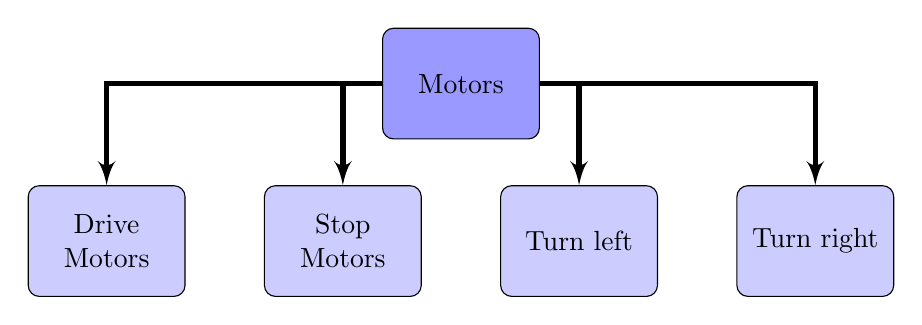
\begin{tikzpicture}[node distance = 2cm, auto]
	\tikzstyle{block} = [rectangle, draw, fill=blue!20, 
	text width=5em, text centered, rounded corners, minimum height=4em]
	\tikzstyle{line} = [draw, -latex', line width =2pt]
	% Place nodes
	\node [block,  fill=blue!40] (motors) {Motors};
	\node [block, below of=motors, xshift=-1.5cm] (stop) {Stop Motors};
	\node [block, left of=stop, node distance = 3 cm] (drive) {Drive Motors};
	\node [block, below of=motors, xshift=1.5cm] (left) {Turn left};
	\node [block, right of=left,  node distance = 3 cm] (right) {Turn right};
	% Draw edges
	\path [line] (motors) -| (drive);
	\path [line] (motors) -| (stop);
	\path [line] (motors) -| (left);
	\path [line] (motors) -| (right);
	\end{tikzpicture}
	\caption{Functions for controlling motors}
	\label{fig:motor_structure}
\end{figure}

Main function is to drive motors was implemented by sending  \textit{linear} and \textit{angular} (i.e. \textit{speed} and \textit{turn}) values, while turn functions are only using angular speed to turn around the given direction. Finally, stopping function request zero linear and zero angular speeds.

\paragraph{Controlling encoders}

For controlling the encoders, registers 2-9 and 16, listed in a table \ref{table:md25}, are used.
Manipulating the mentioned registers, 4 main controlling functions were implemented, which are presented in figure \ref{fig:encoder_structure}.
\begin{figure}[!ht]
	\centering
	\begin{tikzpicture}[node distance = 2cm, auto]
	\tikzstyle{block} = [rectangle, draw, fill=blue!20, 
	text width=5em, text centered, rounded corners, minimum height=4em]
	\tikzstyle{line} = [draw, -latex', line width =2pt]
	% Place nodes
	\node [block, fill=blue!40] (encoders) {Encoders};
	\node [block, below of=encoders, xshift=-1.5cm] 	(rleft) {Read right encoder};
	\node [block, left of=stop, node distance = 3 cm] 	(lleft) {Read left encoder};
	\node [block, below of=encoders, xshift=1.5cm] 	(reset) {Reset both encoders};
	\node [block, right of=left,  node distance = 3 cm] (angle) {Get robot heading};
	% Draw edges
	\path [line] (encoders) -| (rleft);
	\path [line] (encoders) -| (lleft);
	\path [line] (encoders) -| (reset);
	\path [line] (encoders) -| (angle);
	\end{tikzpicture}
	\caption{Functions for manipulating encoders }
	\label{fig:encoder_structure}
\end{figure}

Getting values of encoders or resetting counts included only reading/sending the values from  $I^2C$ bus command register.
Robot \textit{heading} calculation is implemented using two formulas stated in equations \ref{eq:rb_rad-pc}- \ref{eq:rb_heading},
%$$
%radiansPerCount = \pi* (wheelDiameter/trackWidth) / countsPerRevolution
%$$
%and
%$$
%heading = (countsEncoderRight - countsEncoderLeft) * radiansPerCount
%$$ 

\begin{eqnarray}
rad_{pc}  = & \pi \cdot \frac{ d_{wheel} }{ d_{track} } / c_{pr}	,
\label{eq:rb_rad-pc}
\\
\theta_{h} = & (ce_{r} - ce_{l} ) \cdot rad_{pc} ,
\label{eq:rb_heading}
\end{eqnarray}
where 
\begin{itemize}
	\item $rad_{pc}$ - radians per one encoder count,
	\item $d_{wheel}$ - wheel diameter,
	\item $d_{track}$ - track width (or distance between the wheels), %as in figure \ref{fig:rb_wheel_graph},
	\item $c_{pr}$ - encoder counts per output shaft (wheel) turn,
	\item $ce_{r}$ - right encoder counts,
	\item $ce_{l}$ - left encoder counts,
	\item $\theta_{rh}$ - robot heading in radians.
\end{itemize}

Knowing our system constant parameters from robot model shown in figure \ref{fig:rb_wheel_graph},
$$
d_{track} = 224 (mm), \ d_{wheel}=100 (mm), \ c_{pr}=360,
$$
radians per one encoder count can be expressed as
$$
rad_{pc}  = \frac{\pi}{360}\cdot \frac{ 100 }{ 224 } = \frac{\pi}{180}\cdot \frac{ 50 }{ 224 }.
$$

\begin{figure}[!ht]
	\centering
	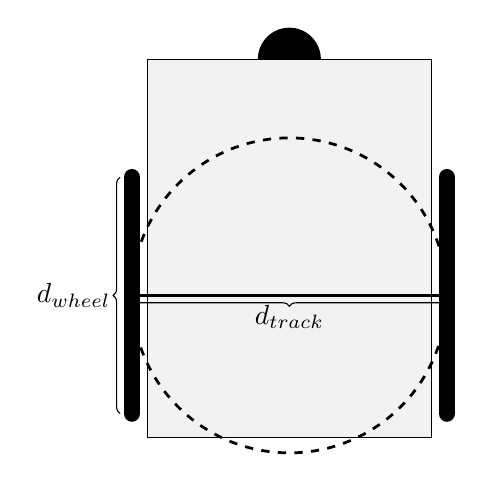
\begin{tikzpicture}
	\def\whDist{2}
	\def\whRad{1.5}
	\def\thirdWheel{3}
	\def\rectBound{0.3}
	
	% wheels
	\draw[line width=6pt, line cap=round] (-\whDist, -\whRad) -- (-\whDist, \whRad);
	\draw[line width=6pt, line cap=round] (\whDist, -\whRad) -- ( \whDist, \whRad);
	%third wheel circle
	\fill[line width = 1pt]  (0, \thirdWheel) circle (0.4);
	
	%robot box
	\draw[fill=gray!10] (-\whDist+0.2, -\whRad-\rectBound) rectangle (\whDist-0.2, \thirdWheel);
	
	% robot circle
	\draw[line width = 1pt, dashed]  (0, 0) circle (\whDist);
	
	%axis between wheels
	\draw[line width = 1pt]  (-\whDist, 0) -- (\whDist, 0);
	%distance decoration
	\draw[ decoration={brace}, decorate] (-\whDist-0.15, -\whRad) -- (-\whDist-0.15, \whRad) node[pos=0.5, anchor=east, ] {$d_{wheel}$};
	%wheel decoration
	\draw[ decoration={brace, mirror, raise=0.05cm}, decorate] (-\whDist, 0) -- (\whDist, 0) node[pos=0.5, anchor=north] {$d_{track}$};
	
	\end{tikzpicture}
	\caption{Robot wheel positioning}
	\label{fig:rb_wheel_graph}
\end{figure}
% optional new page
% to adjust figure
Assuming that our requirement is angle in degrees
$$
\theta_{dh} =  \frac{180}{\pi} \theta_{rh},   
$$
equation \ref{eq:rb_heading} can be simplified and robot heading in degrees can be calculated as
\begin{align*}
\theta_{dh} 
& = \frac{180}{\pi} (ce_{r} - ce_{l} ) \cdot rad_{pc} 								\\
& = \frac{180}{\pi} (ce_{r} - ce_{l} )   \frac{\pi}{180}\cdot \frac{ 50 }{ 224 } 	\\
& = (ce_{r} - ce_{l} ) \cdot \frac{ 50 }{ 224 } 									\\
& \Longrightarrow \\
\theta_{dh}
& = (ce_{r} - ce_{l} ) \cdot \frac{ d_{wheel} }{ 2\cdot d_{track} } .
\end{align*}

Having the left and right encoder counts, the latter equation allows to estimate wheeled robot's heading.
As one knows, dead reckoning is subject to cumulative errors, however in this case, such system position tracking is not implemented. And long-time accumulative errors do not affect turning robot the requested angle, since not the actual accumulative encoder values are used, but only the difference between encoder counts before requesting an action and after.



\subsubsection{Vision module}

The task of vision subsystem is to handle the image data acquired from Raspbery Pi camera. This handling includes two basic subtasks: sign detection and sign recognition.

Three basic signs detected and recognized by the system are shown on figure below.

-----------(color images of all three signs taken by camera)

Different methods and challenges encountered in vision module are described and discussed separately in the following chapters of the report.

\subsubsection{Thresholding}

The first and the most intuitive approach to sign detection procedure was simple color thresholding, since signs which had to be detected are purely red.

The initial choice for color thresholding was HSV color space. Ranges of H (hue), S (saturation) and V (value) channels are [0,180], [0, 255] and [0, 255], respectively. In order to segment only red color, values of H (hue) channel greater than 170 and lower than 10 were used, since this range represents the band of red color. Additionally, too dark (V $ < $ 40), to bright (V $ > $ 220) and non-saturated pixels (S $ < $ 40) were rejected to improve the quality of segmentation. Results are shown on the figure ~\ref{fig:color-spaces}.

\begin{figure}[th!]
	\centering
	\begin{subfigure}[b]{0.3\textwidth}
		\centering
	\includegraphics[scale=0.33]{thresholding-raw.png}
	\subcaption{Raw camera input}
	\end{subfigure}
	\begin{subfigure}[b]{0.3\textwidth}
		\centering
		\includegraphics[scale=0.7]{thresholding-hsv.png}
		\subcaption{HSV color space}
	\end{subfigure}
	\begin{subfigure}[b]{0.3\textwidth}
		\centering
		\includegraphics[scale=0.7]{thresholding-YCrCb.png}
		\subcaption{YCrCb color space}
	\end{subfigure}
	\caption{Comparison of color spaces used for thresholding}
	\label{fig:color-spaces}
\end{figure}

After some testing, YCrCb color space proved to give better results for segmentation, as shown on figure above. As a result, YCrCb color space was used in final implementation.

Usage of IR camera did not affect the recognition quality of the thresholding procedure in regular, normal lighting conditions. On the other hand, it drastically increased the accuracy in low lighting conditions, which is described in Hardware section of the report.

The biggest connected component (blob) int he thresholded image is considered to be a sign. Bounding box of the biggest blob determined the area of the thresholded image to be passed in as an input to the sign classification module. 

\subsection{Classification of the signs using statistical moments}

Taking into consideration the relatively low computational power of the hardware platform used to develop the system, priority for the chosen sign classification algorithm was low complexity.

After some thorough analysis of the available option, statistical moments proven to be the best option.

For an arbitrary binary (i.e. thresholded) input image system can compute statistical moments of desired order. The moment of importance in case of sign classification was center of mass or first order moment. It can be thought of average coordinate of all white pixels for both axes.

\begin{figure}[th!]
	\centering
	\begin{subfigure}[b]{0.25\textwidth}
		\centering
		\includegraphics[scale=0.55]{moments-arrow-raw.png}
		\subcaption{Raw camera input}
	\end{subfigure}
	\begin{subfigure}[b]{0.25\textwidth}
		\centering
		\includegraphics[scale=0.8]{moments-arrow-segm.png}
		\subcaption{Arrow}
	\end{subfigure}
	\begin{subfigure}[b]{0.2\textwidth}
		\centering
		\includegraphics[scale=0.8]{moments-cross-segm.png}
		\subcaption{Cross}
	\end{subfigure}
	\begin{subfigure}[b]{0.2\textwidth}
		\centering
		\includegraphics[scale=0.9]{moments-circle-segm.png}
		\subcaption{Circle}
	\end{subfigure}
	\caption{Visual cues for sign classification using statistical moments}
	\label{fig:statistical-moments}
\end{figure}

Figure \ref{fig:statistical-moments} demonstrates intuition behind visual cues used for discrimination of three different types of signs. By computing the distance of center of the mass (green rectangle) and center of the cropped image segment where the sign was detected (blue rectangle) we can perform initial discrimination between \textbf{arrow} and \textbf{rest two signs}. Distance is going to be close to zero in case of cross and circle since object are symmetrical around two mutually normal axes. Arrow is not symmetrical around one axis, so it's center of the mass will be slightly shifter towards the tip of the arrow and this is the property used to distinguish an arrow from the circle and cross.
Table \ref{tab:moments} shows average distance of center of the mass from image center proportional to cropped image size. Clear observation is that thresholding this distance to 10 $\%$ can give is pretty good estimate of probability that sign belongs to arrow class.

If this distance is close to zero, additional step is needed to determine is the observed sign cross or circle. Approach used in this step was investigation of zero-order moment, which gives the number of white pixels in the image. By taking the ratio of zero order moment and total number of pixels of sign area, we can distinguish between cross and circle. Intuition behind this metric lies in the fact that circle has bigger surface than cross of the same bounding box size, so the percentage of space it occupies in the cropped image area where the sign is going to be larger than if it was cross. Table \ref{tab:moments} gives suitable value of threshold of 70 $\%$.

\begin{table}[th!]
\centering
\begin{tabular}{l*{2}{c}r}
	Sign class			& Distance of first moment & Ratio of second order moment  \\
	\hline
	Arrow 				& 18.41 & 56.44  \\
	Cross            	& 1.39 & 54.20  \\
	Circle           	& 0.97 & 89.63  \\
\end{tabular}
\caption{Numerical values of statistical moments given in $\%$ wrt. image size}
\label{tab:moments}
\end{table}

Images of all three signs with drawn moments and numerical explanation of distinction between those three

\subsection{Neural network classifier}

Justification of usage neural networks.

Very brief theoretical background.

Description of the way how we train it on images (raw pixel values, segmentation pixels, hu-moments as inputs, etc)

Description of tested recognition method (sliding window, random, ...)

Performance comparison with previous method.

\subsection{Arrow angle calculation}

After sign has been classified as arrow, additional step needs to be performed in order to extract the arrow angle relative to the orientation of the robot at the moment of observation.

Description of the initial way (using moments) and failing scenarios. 

Idea of using line fitting, with slight theoretical background and results.

\subsection{Solving partial occlusion and re-detection}

Explanation of problem of partial occlusion and re-detection, when does it happen and why we want to handle it.

Explanation of perceptive area and proximity area.





\section{ Final setup }
During this section the final setup of the robot will be reviewed. First the differences between the initial and the final robot setup will be explained, in terms of hardware, and second the results obtained with it, trying to discuss a bit the reason of them.

\subsection{Innovations in setup (hardware)}

Mainly the innovations on hardware can be divided in two different parts, the ones that are helping the \textit{vision module}, and the ones that are for providing feedback or interaction with the children. The first group includes the new near-IR camera and the IR LED. The second group contains the button and the speaker.

The aim of the first group is to boost the performance of the \textit{vision module}. Mainly it is focused in the use of IR lighting, with the addition of IR LED and the replacement of the regular camera by a near-IR one. Also the position of the camera has been changed in order to increase the \textit{field of view}.

The second group, as said above, tries to improve the experience of the children by adding interaction. The button will allow to start and stop the program when needed. Even it is quite simple it is important to do such action so the robot does not need to be connected to the computer in order to initialize the program again. The speaker will provide sound feedback. For example in the case of the button it will play a short sound so the children know when the robot has started the program or it has closed it.


\subsection{Results and discussion}

In this subsection the results obtained during the different tests will be presented. Some comparison with old and new methods will be reviewed in order to see the improvements done and the performance of the current program. 

One of the first things that was implemented in the \textit{vision module} was the angle detection of the arrow. As explained in previous sections firstly it was using the center of mass of the contour and the center of the rectangle in order to get the angle. This method had a lot of error and it was producing a deviation of $\pm 20º$ according to the real value. Also the angle computed was changing very fast in this range and it was difficult to obtain a clear measure. In order to improve that a new method was designed which fit a line along the arrow. This solution is really easy to implement and the results shows that the deviation is only $\pm 3º$ with respects of the real value. With this little improvement the performance of the angle detection gets increased, thus the turns of the robot are much precise with the direction pointed by the arrow.

One of the biggest problems is the classification of the signs. This is probably one of the points that should be improved if future work is done in the robot. In the current setting the robot is able to distinguish easily between the cross and the circle because of the \textit{fill ratio}. However the arrow is more difficult to detect leading up to a $20\%$ of \textit{false negatives}. This means that every five times and arrow is shown to the robot one is classified as another sign. This result may vary depending on the lighting conditions although the IR signals can avoid loosing precision in low light conditions. The lack of accuracy of the center of mass and center of rectangle method is leading to this \textit{false negatives} because sometimes this two points are not split enough and the sign is not classified as an arrow. Probably getting some information about the shape of the bounding box would help in order to improve the arrow detection.

It has been also detected that when the arrow is placed pointing near $90º$ either left or right, the detections are much more better than when the arrow is pointing forward with respects to the current angle of the robot. This is probably caused by the perspective of the camera with respects to the ground plane. Whenever the arrow is pointing forward the deformation due to the perspective is causing the center of mass to be very close to the center of the bounding box. More stylized arrows would probably solve the problem by shifting a bit the center of mass towards the direction of the arrow. In this case it would be difficult to use the shape of the bounding box since an arrow in perspective is seen most of the times in a shape similar to a square.

As seen in table \ref{tab:cam_perf} of the hardware section the camera of the Raspberry Pi is able to give up to 18 \textit{frames per second}. However this speed is impossible to achieve due to the high demand on computational resources of the \textit{vision module}. The tests during most of the implementation were always performed using \textit{graphical user interface} on the Raspberry Pi and showing results on an external display. This was the unique way to check that everything was working perfectly on the RPi since all the code was developed on \textit{Visual Studio} in \textit{Windows}. The \textit{fps} achieved with this configuration were very close to 5, in an image of $160x120$. However the final version of the program does not need to show anything on screen since the robot will be moving around a room with no connection to external screens or other computers. This allows to avoid the execution of all the lines in the code that refers to the \textit{GUI}, mainly showing images and plotting lines, rectangles, proximity areas, etc. 



\section{Problems encountered}


\subsection{Limitations}

The hardware of the Raspberry Pi doesn't allow to perform any intensive
computations, so it is necessary to balance between robustness and
computational time.

\subsection{Hardware}

\begin{itemize}
  	\item The overall performance of the Raspberry Pi showed satisfactory
  	results for the given problem.
  	\item The reliability of the WiFi connection is low - the board can lose
  connection to WiFi dongle at any time. Loss of the connection can also be caused by an
external disturbance (e.g. sharp velocity changes).
	\item RPi Camera Module is very sensitive to static electricity.
	\item Sharp increase of the torque in the motors can cause the voltage drop in
	the power supply that will lead to board shutdown
\end{itemize}

Power plug issues (?)

\subsection{Software}

\begin{itemize}
  \item OpenCV takes almost 9 hours to compile. (Include OpenCV compilation
  guide?)
  \item No Software is available for the GPU access
\end{itemize}

It was necessary to synchronize the software development for the board between
the group participants, so the development process was done using Microsoft
Visual Studio 2013. This lead to the necessity of making the code
cross-compilable. Remote access to RPi is established via SSH and an xServer.
Remote Desktop Environment was provided by MobaXTerm software.

\section{Further improvements}



\subsection{Robustness of sign classification}

Current sign classification approach is computationally inexpensive and has simple implementation and execution. Price paid for these benefits is low robustness, meaning that there are times when robot detects some other red object's shape as one of the three signs that it needs to classify.

In order to avoid these issues a more robust classifier is needed. Approach using artificial neural networks, Support Vector Machines or any other machine learning technique would require training classifiers on another (more powerful) CPU and loading trained classifier to the robot just for the purposes of classification.

\subsection{Complex game rules and sign diversity}

Current rules for interaction with robot rely only on couple of simple actions and available signs. Software control architecture is built in a way modular way, which enables easy addition of the new signs under assumption of robust classifier able to distinguish between all currently known signs and newly added one.

Expanding set of available signs could enrich the game experience by introducing new objectives, goals and obstacles for the children to play with.

\subsection{Hardware improvements}

Although system is currently able to perform all desired tasks, a \textit{more powerful processing hardware would make it faster, more responsive} and, thus, more fun for children to play with. Having only 6 FPS from camera limits the maximum velocity of robot movement as well, so games would look more dynamic if robot was able to move faster. 

It would, also, enable usage of more advanced and, at the same time, more robust algorithms for image processing. This would \textit{remove some limitations and conditions} put on the usage of the robot, like camera pointing only towards ground (floor) plane, maximum distance of sign placement, sign shape and color restrictions, etc.

\textit{More sensors} would enrich engagement of the children as well by providing diverse set of ways to interact with the robot. 




Example of cite and referencing:\cite{craig2005introduction}

\clearpage

\printbibliography

\end{document}